% arara: lualatex: { synctex: on, shell: off }
% arara: biber
% arara: lualatex: { synctex: on, shell: off }
% arara: sumatrapdf
\documentclass[../main.tex]{subfiles}
\begin{document}

The fast sampling system (FSS) used in this work is a commercial system supplied by
SME-Tec Gmbh. from Germany. The FSS is composed of two parts, the gas sampling valve
(GSV) and the Controller. A photo of the GSV is shown in \cref{fig:gsv-photo}.
Gases are admitted from the reaction chamber into the heated carrying tubes
through the poppet-style valve on the left of the GSV. The sampled gases are then
conducted through the GSV outlet into a sampling bottle.

A schematic of the GSV assembly is shown in \cref{fig:gsv-assem-schematic}.
The GSV is mounted to the RCM by a custom-made end plug. The reaction chamber
is sealed by an O-ring on the small- and large-diameter portions of the GSV.
The depth that the GSV is inserted into the reaction chamber is adjustable
by adding or removing shims in the end plug assembly. The insertion depth
is chosen so that the tip of the GSV is outside the boundary layer on the
end wall.

\begin{figure}
    \begin{floatrow}
        \ffigbox
            {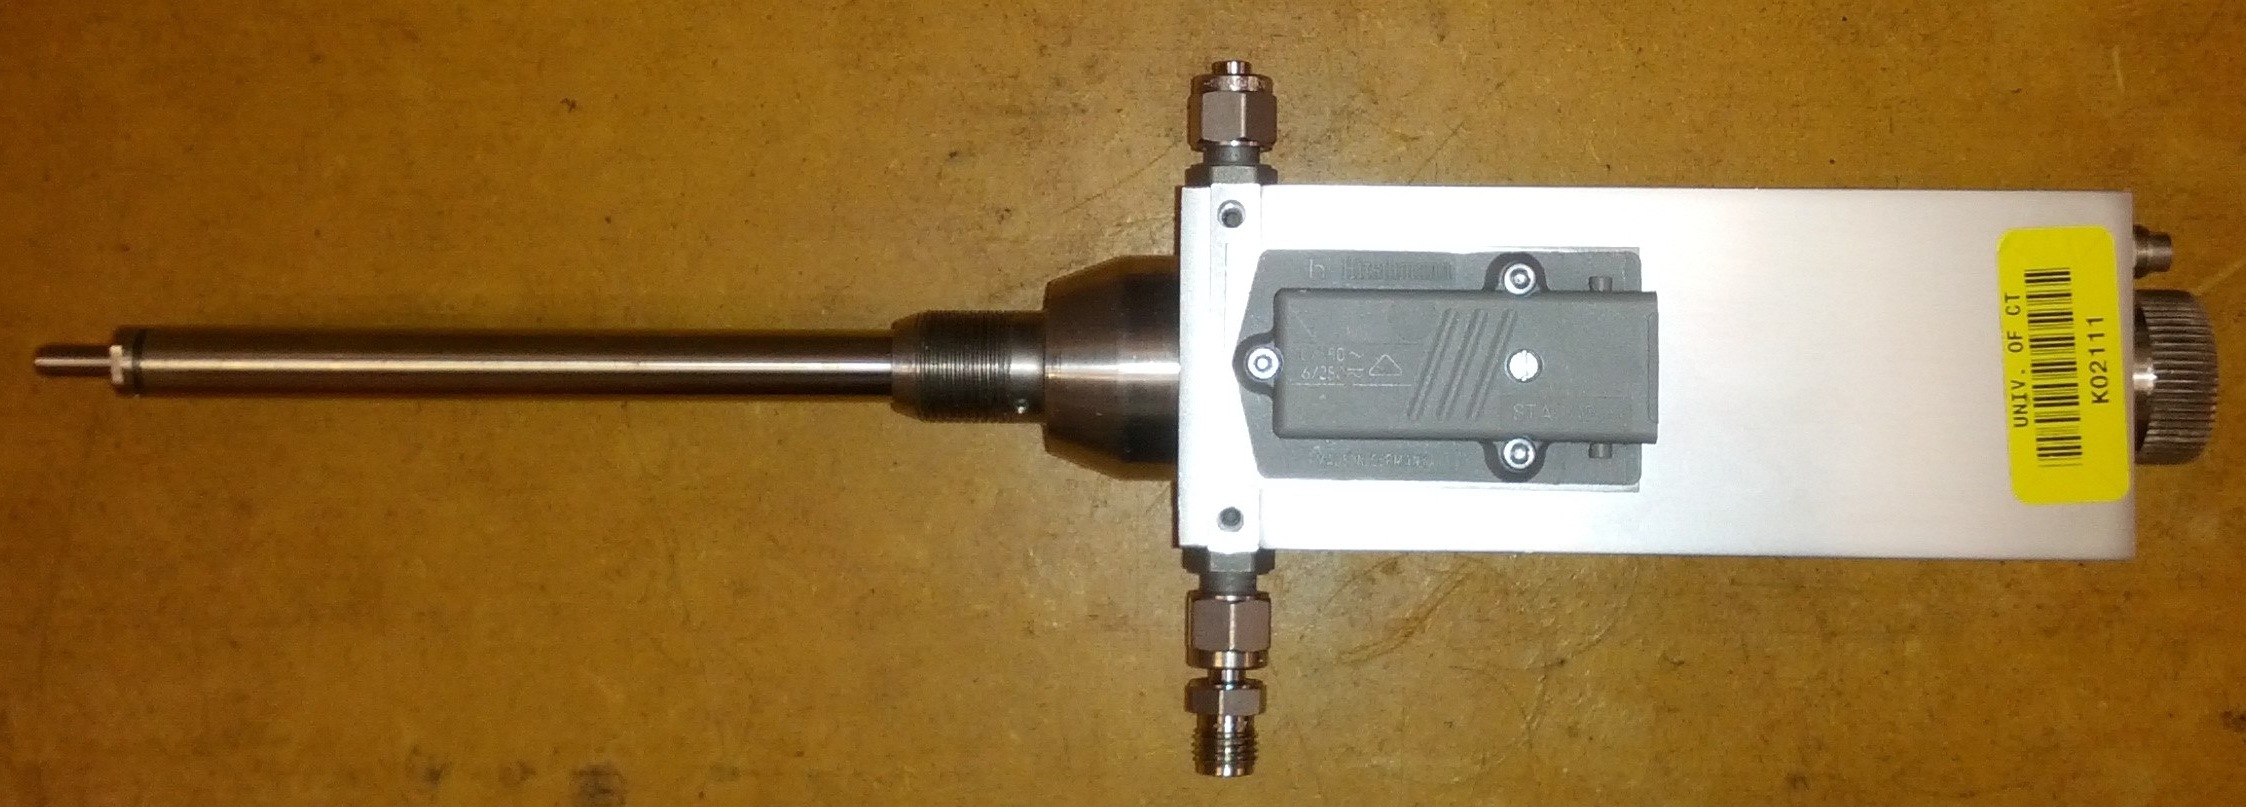
\includegraphics[width=7.9cm]{B-Fast-Sampling-System/gsv-photo}}
            {\caption{Photo of the GSV prior to installation in the RCM. Samples
            enter the valve from the left and are removed through the ports in the
            center of the GSV.}
            \label{fig:gsv-photo}}
        \ffigbox
            {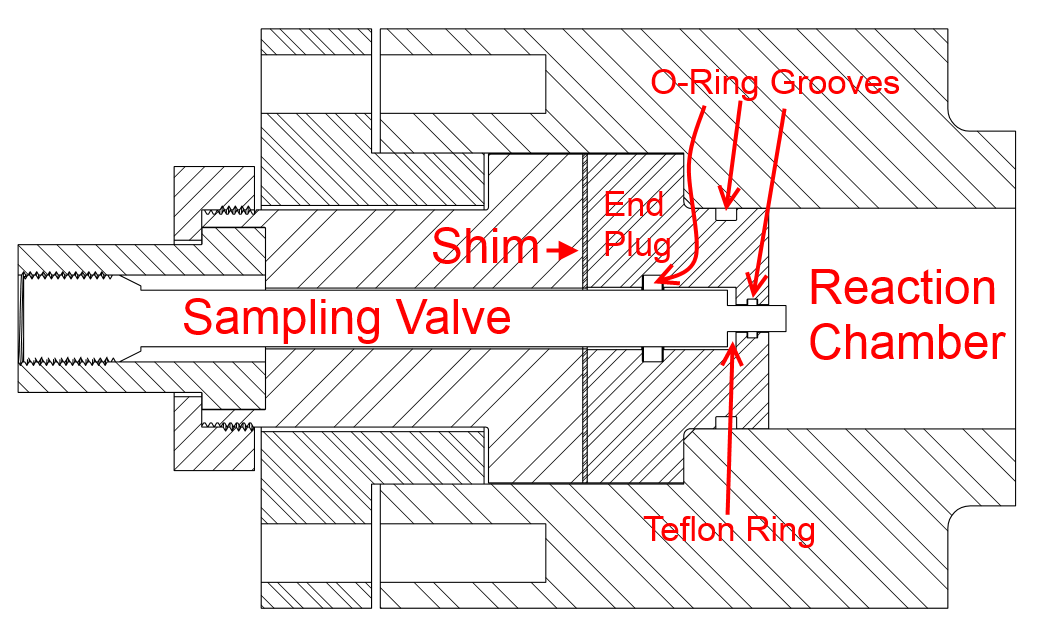
\includegraphics[width=7.9cm]{B-Fast-Sampling-System/gsv-assem-schematic}}
            {\caption{Schematic of the GSV assembled into the reaction chamber showing
            the position of the sealing o-rings and the protrusion of the poppet face.}
            \label{fig:gsv-assem-schematic}}
    \end{floatrow}
\end{figure}

The portion of the GSV protruding into the reaction chamber has minimal
effect on the homogeneity of the reaction chamber. Moreover, the removal of
samples has minimal effect on the measured ignition delay.
This has been verified experimentally by measuring the ignition delay with
and without the GSV present, and with and without sampling occurring.
In both cases, the difference in ignition delay was statistically insignificant
for $\alpha=0.05$.

Tests of the ignition delay with and without the valve, and with and
without sampling are shown in \cref{fig:gsv-pressure}. It can be seen
that the pressure traces follow each other closely, including through the
ignition event, indicating that the presence of the valve and the
activation of the valve to remove a sample do not substantially disturb
the ignition process.

\begin{figure}
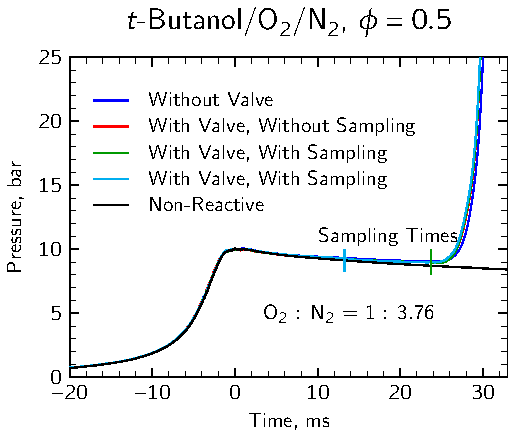
\includegraphics[width=9cm]{B-Fast-Sampling-System/gsv-pressure}
\caption{Representative pressure traces from RCM experiments with and
without the GSV present, and with and without sampling occurring. Two
sampling times are shown. The corresponding non-reactive pressure trace
is also shown.}
\label{fig:gsv-pressure}
\end{figure}

The close-open-close (COC) cycle of the GSV is controlled by a mass-spring
system shown in \cref{fig:gsv-magnet-section}. The poppet face is connected
to a rod running the length of the
GSV and connected to the mass at the rear of the valve. To open the poppet,
the mass is accelerated forward by passing current through the coil around
the mass. The rod is also
connected to a spring that is used to restore the poppet to its original
position after being extended.

\begin{figure}
    \ffigbox{%
        \begin{subfloatrow}
            \ffigbox[\FBwidth]
                {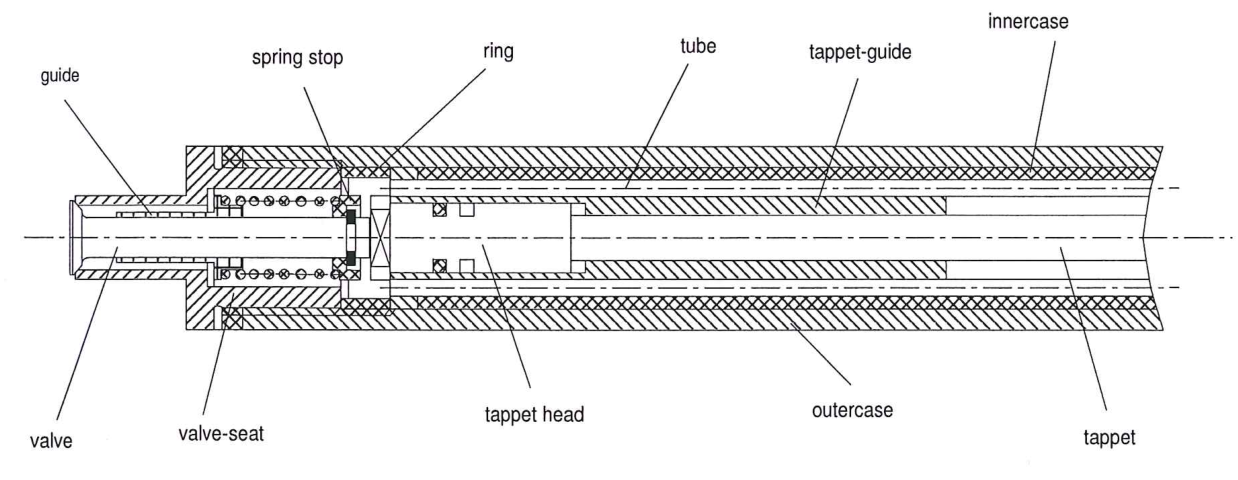
\includegraphics[width=13cm]{B-Fast-Sampling-System/tube-valve-section}}
                {\caption{Front section of the GSV containing the sample transfer tubes
                and the poppet valve that is inserted into the reaction chamber}
                \label{fig:gsv-tube-valve-section}}
        \end{subfloatrow}%
        \par
        \begin{subfloatrow}%
            \ffigbox[\FBwidth]
                {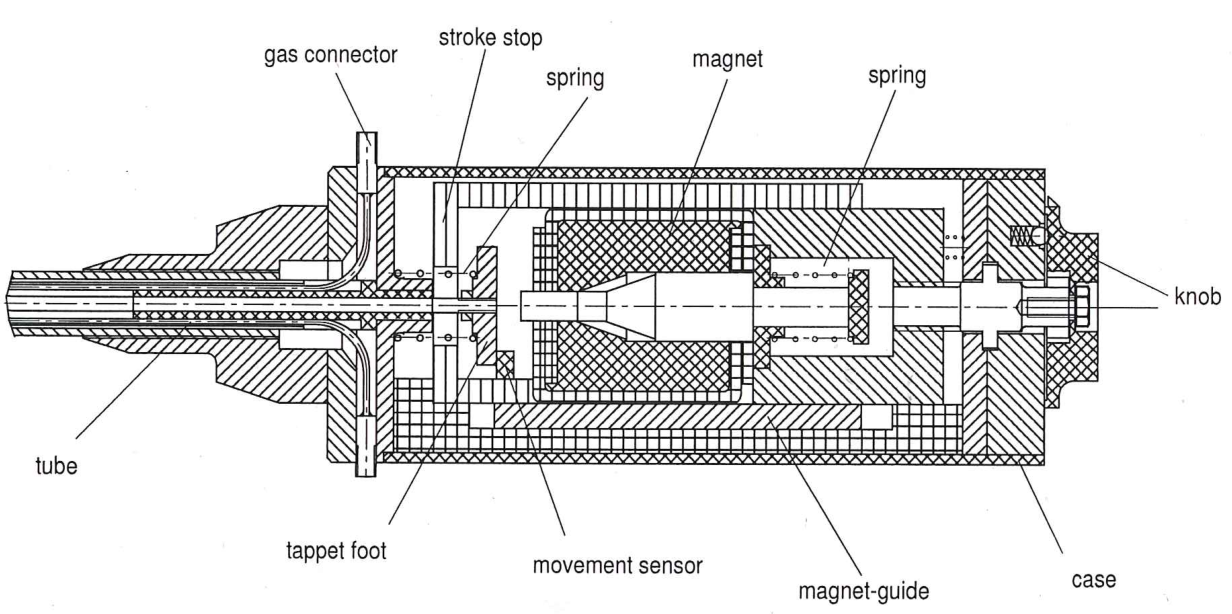
\includegraphics[width=13cm]{B-Fast-Sampling-System/magnet-section}}
                {\caption{Rear section of the GSV containing the driving magnet and
                sample extraction fittings.}
                \label{fig:gsv-magnet-section}}
        \end{subfloatrow}}
        {\caption{Schematic of the front and rear portions of the GSV. Images courtesy
        SMETec GMBH.}
        \label{fig:gsv-schematic}}
\end{figure}

The GSV has an adjustable COC time, by adjusting the
distance the plate is allowed to move. Furthermore, the GSV has the ability
to measure the displacement of the mass, allowing the direct measurement of
the COC time and the absolute time of opening.

The GSV controller is triggered by a \SI{5}{\volt} signal from the cDAQ.
The timing of the trigger signal is controlled by the LabView VI. The pressure
signal from the reaction chamber is read from the cDAQ in \SI{1}{\milli\second}
chunks in a loop. On each loop iteration, the maximum pressure is checked
against a desired trigger pressure; when the reaction chamber pressure exceeds
the trigger pressure, the cDAQ sends the trigger to the GSV controller. The
GSV controller has an adjustable delay (\SIrange{4.5}{70}{\milli\second}) that
is used to control the timing of the opening of the GSV during the induction period.
The absolute opening time of the GSV is thus dependent on three parameters:
\begin{enumerate}
\item The cable delays from the PC to the cDAQ; from the cDAQ to the GSV
      controller; and from the GSV controller to the GSV itself
\item The processing time of the LabView VI
\item The delay set in the GSV controller.
\end{enumerate}

The absolute opening time of the GSV is measured by
the signal sent from the GSV to the controller (and thence to the cDAQ).
This signal is shown in \cref{fig:gsv-voltage}. The time that
the cDAQ sent the trigger signal to the GSV controller is set to be the
zero time; \cref{fig:gsv-voltage} thus demonstrates the
repeatability of the delay (within \SI{1}{\milli\second}) in 
GSV motion relative to the trigger signal.

The COC time is measured as the width of the first peak in the
GSV valve signal in \cref{fig:gsv-voltage}. \Cref{fig:gsv-voltage} 
shows the repeatability of the COC time as the width of the first 
peak for the two sampling times corresponds closely between runs.

\begin{figure}
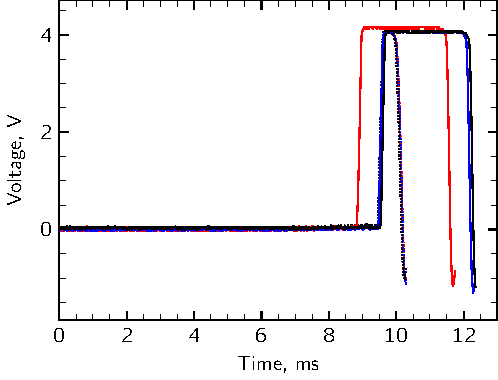
\includegraphics[width=11cm]{B-Fast-Sampling-System/gsv-voltage}
\caption{Representative voltage traces from three runs each of two
COC times: dotted: \SI{0.8}{\milli\second}; solid: \SI{2.5}{\milli\second}.}
\label{fig:gsv-voltage}
\end{figure}

Further characterization work is required to determine the temperature
drop of the gas as it enters the GSV and to ensure that the GSV tip
protrudes beyond the boundary layer. In addition, an experimental
procedure must be developed to integrate the GSV with the GC/MS analysis.

\end{document}
